% Options for packages loaded elsewhere
\PassOptionsToPackage{unicode}{hyperref}
\PassOptionsToPackage{hyphens}{url}
%
\documentclass[
  man,floatsintext]{apa6}
\usepackage{amsmath,amssymb}
\usepackage{lmodern}
\usepackage{iftex}
\ifPDFTeX
  \usepackage[T1]{fontenc}
  \usepackage[utf8]{inputenc}
  \usepackage{textcomp} % provide euro and other symbols
\else % if luatex or xetex
  \usepackage{unicode-math}
  \defaultfontfeatures{Scale=MatchLowercase}
  \defaultfontfeatures[\rmfamily]{Ligatures=TeX,Scale=1}
\fi
% Use upquote if available, for straight quotes in verbatim environments
\IfFileExists{upquote.sty}{\usepackage{upquote}}{}
\IfFileExists{microtype.sty}{% use microtype if available
  \usepackage[]{microtype}
  \UseMicrotypeSet[protrusion]{basicmath} % disable protrusion for tt fonts
}{}
\makeatletter
\@ifundefined{KOMAClassName}{% if non-KOMA class
  \IfFileExists{parskip.sty}{%
    \usepackage{parskip}
  }{% else
    \setlength{\parindent}{0pt}
    \setlength{\parskip}{6pt plus 2pt minus 1pt}}
}{% if KOMA class
  \KOMAoptions{parskip=half}}
\makeatother
\usepackage{xcolor}
\IfFileExists{xurl.sty}{\usepackage{xurl}}{} % add URL line breaks if available
\IfFileExists{bookmark.sty}{\usepackage{bookmark}}{\usepackage{hyperref}}
\hypersetup{
  pdftitle={Measuring individual differences in the understanding of gaze cues across the lifespan},
  pdfauthor={Julia Prein1, Manuel Bohn1, Luke Maurits1, Steven Kalinke1, \& Daniel M. Haun1},
  pdflang={en-EN},
  pdfkeywords={social cognition, individual differences, gaze cues, psychometrics},
  hidelinks,
  pdfcreator={LaTeX via pandoc}}
\urlstyle{same} % disable monospaced font for URLs
\usepackage{longtable,booktabs,array}
\usepackage{calc} % for calculating minipage widths
% Correct order of tables after \paragraph or \subparagraph
\usepackage{etoolbox}
\makeatletter
\patchcmd\longtable{\par}{\if@noskipsec\mbox{}\fi\par}{}{}
\makeatother
% Allow footnotes in longtable head/foot
\IfFileExists{footnotehyper.sty}{\usepackage{footnotehyper}}{\usepackage{footnote}}
\makesavenoteenv{longtable}
\usepackage{graphicx}
\makeatletter
\def\maxwidth{\ifdim\Gin@nat@width>\linewidth\linewidth\else\Gin@nat@width\fi}
\def\maxheight{\ifdim\Gin@nat@height>\textheight\textheight\else\Gin@nat@height\fi}
\makeatother
% Scale images if necessary, so that they will not overflow the page
% margins by default, and it is still possible to overwrite the defaults
% using explicit options in \includegraphics[width, height, ...]{}
\setkeys{Gin}{width=\maxwidth,height=\maxheight,keepaspectratio}
% Set default figure placement to htbp
\makeatletter
\def\fps@figure{htbp}
\makeatother
\setlength{\emergencystretch}{3em} % prevent overfull lines
\providecommand{\tightlist}{%
  \setlength{\itemsep}{0pt}\setlength{\parskip}{0pt}}
\setcounter{secnumdepth}{-\maxdimen} % remove section numbering
% Make \paragraph and \subparagraph free-standing
\ifx\paragraph\undefined\else
  \let\oldparagraph\paragraph
  \renewcommand{\paragraph}[1]{\oldparagraph{#1}\mbox{}}
\fi
\ifx\subparagraph\undefined\else
  \let\oldsubparagraph\subparagraph
  \renewcommand{\subparagraph}[1]{\oldsubparagraph{#1}\mbox{}}
\fi
\newlength{\cslhangindent}
\setlength{\cslhangindent}{1.5em}
\newlength{\csllabelwidth}
\setlength{\csllabelwidth}{3em}
\newlength{\cslentryspacingunit} % times entry-spacing
\setlength{\cslentryspacingunit}{\parskip}
\newenvironment{CSLReferences}[2] % #1 hanging-ident, #2 entry spacing
 {% don't indent paragraphs
  \setlength{\parindent}{0pt}
  % turn on hanging indent if param 1 is 1
  \ifodd #1
  \let\oldpar\par
  \def\par{\hangindent=\cslhangindent\oldpar}
  \fi
  % set entry spacing
  \setlength{\parskip}{#2\cslentryspacingunit}
 }%
 {}
\usepackage{calc}
\newcommand{\CSLBlock}[1]{#1\hfill\break}
\newcommand{\CSLLeftMargin}[1]{\parbox[t]{\csllabelwidth}{#1}}
\newcommand{\CSLRightInline}[1]{\parbox[t]{\linewidth - \csllabelwidth}{#1}\break}
\newcommand{\CSLIndent}[1]{\hspace{\cslhangindent}#1}
\ifLuaTeX
\usepackage[bidi=basic]{babel}
\else
\usepackage[bidi=default]{babel}
\fi
\babelprovide[main,import]{english}
% get rid of language-specific shorthands (see #6817):
\let\LanguageShortHands\languageshorthands
\def\languageshorthands#1{}
% Manuscript styling
\usepackage{upgreek}
\captionsetup{font=singlespacing,justification=justified}

% Table formatting
\usepackage{longtable}
\usepackage{lscape}
% \usepackage[counterclockwise]{rotating}   % Landscape page setup for large tables
\usepackage{multirow}		% Table styling
\usepackage{tabularx}		% Control Column width
\usepackage[flushleft]{threeparttable}	% Allows for three part tables with a specified notes section
\usepackage{threeparttablex}            % Lets threeparttable work with longtable

% Create new environments so endfloat can handle them
% \newenvironment{ltable}
%   {\begin{landscape}\begin{center}\begin{threeparttable}}
%   {\end{threeparttable}\end{center}\end{landscape}}
\newenvironment{lltable}{\begin{landscape}\begin{center}\begin{ThreePartTable}}{\end{ThreePartTable}\end{center}\end{landscape}}

% Enables adjusting longtable caption width to table width
% Solution found at http://golatex.de/longtable-mit-caption-so-breit-wie-die-tabelle-t15767.html
\makeatletter
\newcommand\LastLTentrywidth{1em}
\newlength\longtablewidth
\setlength{\longtablewidth}{1in}
\newcommand{\getlongtablewidth}{\begingroup \ifcsname LT@\roman{LT@tables}\endcsname \global\longtablewidth=0pt \renewcommand{\LT@entry}[2]{\global\advance\longtablewidth by ##2\relax\gdef\LastLTentrywidth{##2}}\@nameuse{LT@\roman{LT@tables}} \fi \endgroup}

% \setlength{\parindent}{0.5in}
% \setlength{\parskip}{0pt plus 0pt minus 0pt}

% Overwrite redefinition of paragraph and subparagraph by the default LaTeX template
% See https://github.com/crsh/papaja/issues/292
\makeatletter
\renewcommand{\paragraph}{\@startsection{paragraph}{4}{\parindent}%
  {0\baselineskip \@plus 0.2ex \@minus 0.2ex}%
  {-1em}%
  {\normalfont\normalsize\bfseries\itshape\typesectitle}}

\renewcommand{\subparagraph}[1]{\@startsection{subparagraph}{5}{1em}%
  {0\baselineskip \@plus 0.2ex \@minus 0.2ex}%
  {-\z@\relax}%
  {\normalfont\normalsize\itshape\hspace{\parindent}{#1}\textit{\addperi}}{\relax}}
\makeatother

% \usepackage{etoolbox}
\makeatletter
\patchcmd{\HyOrg@maketitle}
  {\section{\normalfont\normalsize\abstractname}}
  {\section*{\normalfont\normalsize\abstractname}}
  {}{\typeout{Failed to patch abstract.}}
\patchcmd{\HyOrg@maketitle}
  {\section{\protect\normalfont{\@title}}}
  {\section*{\protect\normalfont{\@title}}}
  {}{\typeout{Failed to patch title.}}
\makeatother

\usepackage{xpatch}
\makeatletter
\xapptocmd\appendix
  {\xapptocmd\section
    {\addcontentsline{toc}{section}{\appendixname\ifoneappendix\else~\theappendix\fi\\: #1}}
    {}{\InnerPatchFailed}%
  }
{}{\PatchFailed}
\keywords{social cognition, individual differences, gaze cues, psychometrics\newline\indent Word count: X}
\usepackage{lineno}

\linenumbers
\usepackage{csquotes}
\usepackage{setspace}
\captionsetup[figure]{font={stretch=1}}
\ifLuaTeX
  \usepackage{selnolig}  % disable illegal ligatures
\fi

\title{Measuring individual differences in the understanding of gaze cues across the lifespan}
\author{Julia Prein\textsuperscript{1}, Manuel Bohn\textsuperscript{1}, Luke Maurits\textsuperscript{1}, Steven Kalinke\textsuperscript{1}, \& Daniel M. Haun\textsuperscript{1}}
\date{}


\shorttitle{Gaze cue understanding}

\authornote{

Correspondence concerning this article should be addressed to Julia Prein, Max Planck Institute for Evolutionary Anthropology, Deutscher Platz 6, 04103 Leipzig, Germany. E-mail: \href{mailto:julia_prein@eva.mpg.de}{\nolinkurl{julia\_prein@eva.mpg.de}}

}

\affiliation{\vspace{0.5cm}\textsuperscript{1} Department of Comparative Cultural Psychology, Max Planck Institute for Evolutionary Anthropology, Leipzig, Germany}

\abstract{%
There must be an abstract of no more than 250 words.
One or two sentences providing a \textbf{basic introduction} to the field, comprehensible to a scientist in any discipline.

Two to three sentences of \textbf{more detailed background}, comprehensible to scientists in related disciplines.

One sentence clearly stating the \textbf{general problem} being addressed by this particular study.

One sentence summarizing the main result (with the words ``\textbf{here we show}'' or their equivalent).

Two or three sentences explaining what the \textbf{main result} reveals in direct comparison to what was thought to be the case previously, or how the main result adds to previous knowledge.

One or two sentences to put the results into a more \textbf{general context}.

Two or three sentences to provide a \textbf{broader perspective}, readily comprehensible to a scientist in any discipline.
}



\begin{document}
\maketitle

\hypertarget{introduction}{%
\section{Introduction}\label{introduction}}

Idea for an opener :)

Developmental psychology is facing a dilemma: many research questions are questions about individual differences, yet, there is a lack of tasks to reliably measure these individual differences. For example \ldots{}

\begin{itemize}
\tightlist
\item
  why is social cognition important
\item
  what methods are currently been used?: wellman
\item
  what are common issues?
\item
  what to aim at. individual differences in developmental psychology
\item
  what characteristics should a new task fulfill? reliable tasks, variation needed, more trials
\item
  goal of the current project: standardized, easy to use continuous methods
\end{itemize}

``Recently, it was suggested that a range of cognitive tasks may reliably measure group differences but not individual differences (Hedge et al., 2018). As cognitive tests are commonly used to make inferences about individuals, it seems a worthwhile pursuit to improve the reliability with which individual differences are assessed using these tests. To judge the success of such pursuits, accurate estimates of reliability are required.'' (Pronk, Molenaar, Wiers and Murre, 2021, p.~1)
``Firstly, reliability is not only a function of task and population sample but also of scoring algorithms.'' (Pronk, Molenaar, Wiers and Murre, 2021, p.~9)
``Hence, we conclude that for the datasets included in our reanalysis, cognitive tasks may well have been able to measure individual differences, but that these differences may be relatively unstable over time (Kopp et al., 2021). In practice, this may make cognitive tasks suitable for cross-sectional research of individual differences, but not for longitudinal research.'' (Pronk, Molenaar, Wiers and Murre, 2021, p.~10)

Rakoczy, H. (2022). Foundations of theory of mind and its development in early childhood. Nature Reviews Psychology, 1--13. \url{https://doi.org/10.1038/s44159-022-00037-z}:
``The way humans view agents, be it others or themselves, differs radically from the way humans view the rest of the world. This difference is because agents feel, perceive and think. Agents see the world from their own subjective perspective and they rationally plan, form intentions and act accordingly. This way of seeing others as rational subjects with individual perspectives on the world is termed theory of mind (ToM).'' (p.~1)
``ToM also has specific real-life consequences. First, the development of ToM competence goes along with general measures of children's peer social skills in early and middle childhood. (\ldots) Second, ToM specifically predicts communicative competence. (\ldots) Third, ToM competence is related to the quality of peer relationships: children with more advanced ToM are rated as more likeable and popular among their peers. Fourth, children who are more proficient at ToM tasks tend to act more prosocially, including comforting, sharing or helping other individuals. Finally, preschool ToM competence predicts achievement in primary school, a relationship that is possibly mediated by social competence, in that preschool ToM abilities enable subsequent social competence development, which in turn contributes to school achievement.'' (p.~2)
``Evidence for an emerging understanding of perception at 9 months of age comes from various sources. For example, children begin to follow the gaze of other agents in systematic and differential ways: they follow an agent's head turn only when the agent can actually see (has their eyes open rather than closed, or wears a transparent rather than an opaque blindfold).'' (p.~2)
Developmental determinants: executive function, language (``that'' complementations), social (SES, siblings, mind-minded parents)
Implicit tasks: ``A third class of implicit ToM tasks is interaction tasks, in which participants are involved in a communicative or cooperative interaction with another agent. This agent forms a mental state (such as a true or false belief regarding the contents of a box) and experimenters measure whether participants spontaneously take the agent's belief into account in their interaction with the agent (for instance by helping or by interpreting the agent's communicative acts accordingly)'' (p.~9)
=\textgreater{} reliable \& valid tasks to assess coherent development of social-cognitive functions

\hypertarget{design-of-our-balloon-finding-task}{%
\section{Design of our balloon finding task}\label{design-of-our-balloon-finding-task}}

\begin{itemize}
\tightlist
\item
  face value of task (or maybe in intro already?)
\end{itemize}

\hypertarget{stimuli}{%
\subsection{Stimuli}\label{stimuli}}

Our newly implemented balloon finding task displays cartoon-like stimuli that are engaging for children and adults alike. An animal character (i.e., agent; sheep, monkey, or pig) is placed centrally in a window. A balloon (i.e., target; blue, green, yellow, or red) is located in front of them. The target then falls to the ground. At all times, the agent's gaze tracks the movement of the target. That is, the pupils and iris of the agent move in a way that their center aligns with the center of the target. While the distance of the target's flight depends on the final location, the target moves at a constant speed. Participants are then asked to locate the target's destination: they respond by touching or clicking onto position on the screen.

To keep participants engaged and interested, the presentation of events is accompanied by cartoon-like effects. Each trial starts with an attention-getter: an eye-blinking sound plays while the pupils and iris of the agent enlarge (increase to 130\%) and change in opacity (decrease to 75\%) for 0.3 sec.~The landing of the target is accompanied by a tapping sound. Once the target landed, the instructor's voice asks ``Where is the balloon?''. After the response is registered, a short plop sound plays and a small orange circle confirms the participants' location choice. If no response got registered within 5 secs after the target landed, an audio prompt reminds the participant to respond.

\hypertarget{trials}{%
\subsection{Trials}\label{trials}}

Before the test trials start, we present four training trials during which participants familiarize themselves with selection positions on the screen. In the first training trial, participants have full visual access to the target flight and the target's end location and are simply asked to click on the visible balloon. In the second and third training trials, participants have partial visual access: they witness the target flight but cannot see the target's end location. They are then asked to click on the invisible balloon, i.e., the location where they saw the target land. In test trials, participants have no visual access to the target flight nor the end location. Participants are expected to use the agent's gaze as a cue to locate the target. The first trial of each type comprises a voice-over description of the presented events. The audio descriptions explicitly state that the agent is always looking at the target (see Appendix for audio script). After these four training and audio guided trials, participants receive 15 test trials. The complete sequence of four training trials and 15 test trials can be administered within 5-10 minutes of testing time.

\hypertarget{study-versions}{%
\subsection{Study versions}\label{study-versions}}

We designed two study versions which can be chosen according to the researchers' need: there is a continuous \emph{hedge} version and a discrete \emph{box} version. Both versions use the same first training trial and then differ in the consecutive training and test trials.
In the \emph{hedge} version, participants have to indicate their estimated target location directly on a hedge (i.e., hedge version).
Here, the dependent variable is imprecision, which is defined as the absolute difference between the target's true x coordinate and the x coordinate of the participant's click.
In the \emph{box} version, participants are asked to click on a box that hides the target. Researchers have the choice of how many boxes are shown: one up to eight boxes can be displayed as potential hiding locations. Here, we use a categorical outcome (i.e., which box was clicked) to calculate the proportion of correct responses.
Note that in the test trials of both study versions, the target flight is covered by a hedge. In the \emph{hedge} version, the hedge then shrinks to a minimum height required to cover the target's end location. In the \emph{box} version, the hedge shrinks completely. The boxes then hide the target's final destination.






\begin{figure}

{\centering 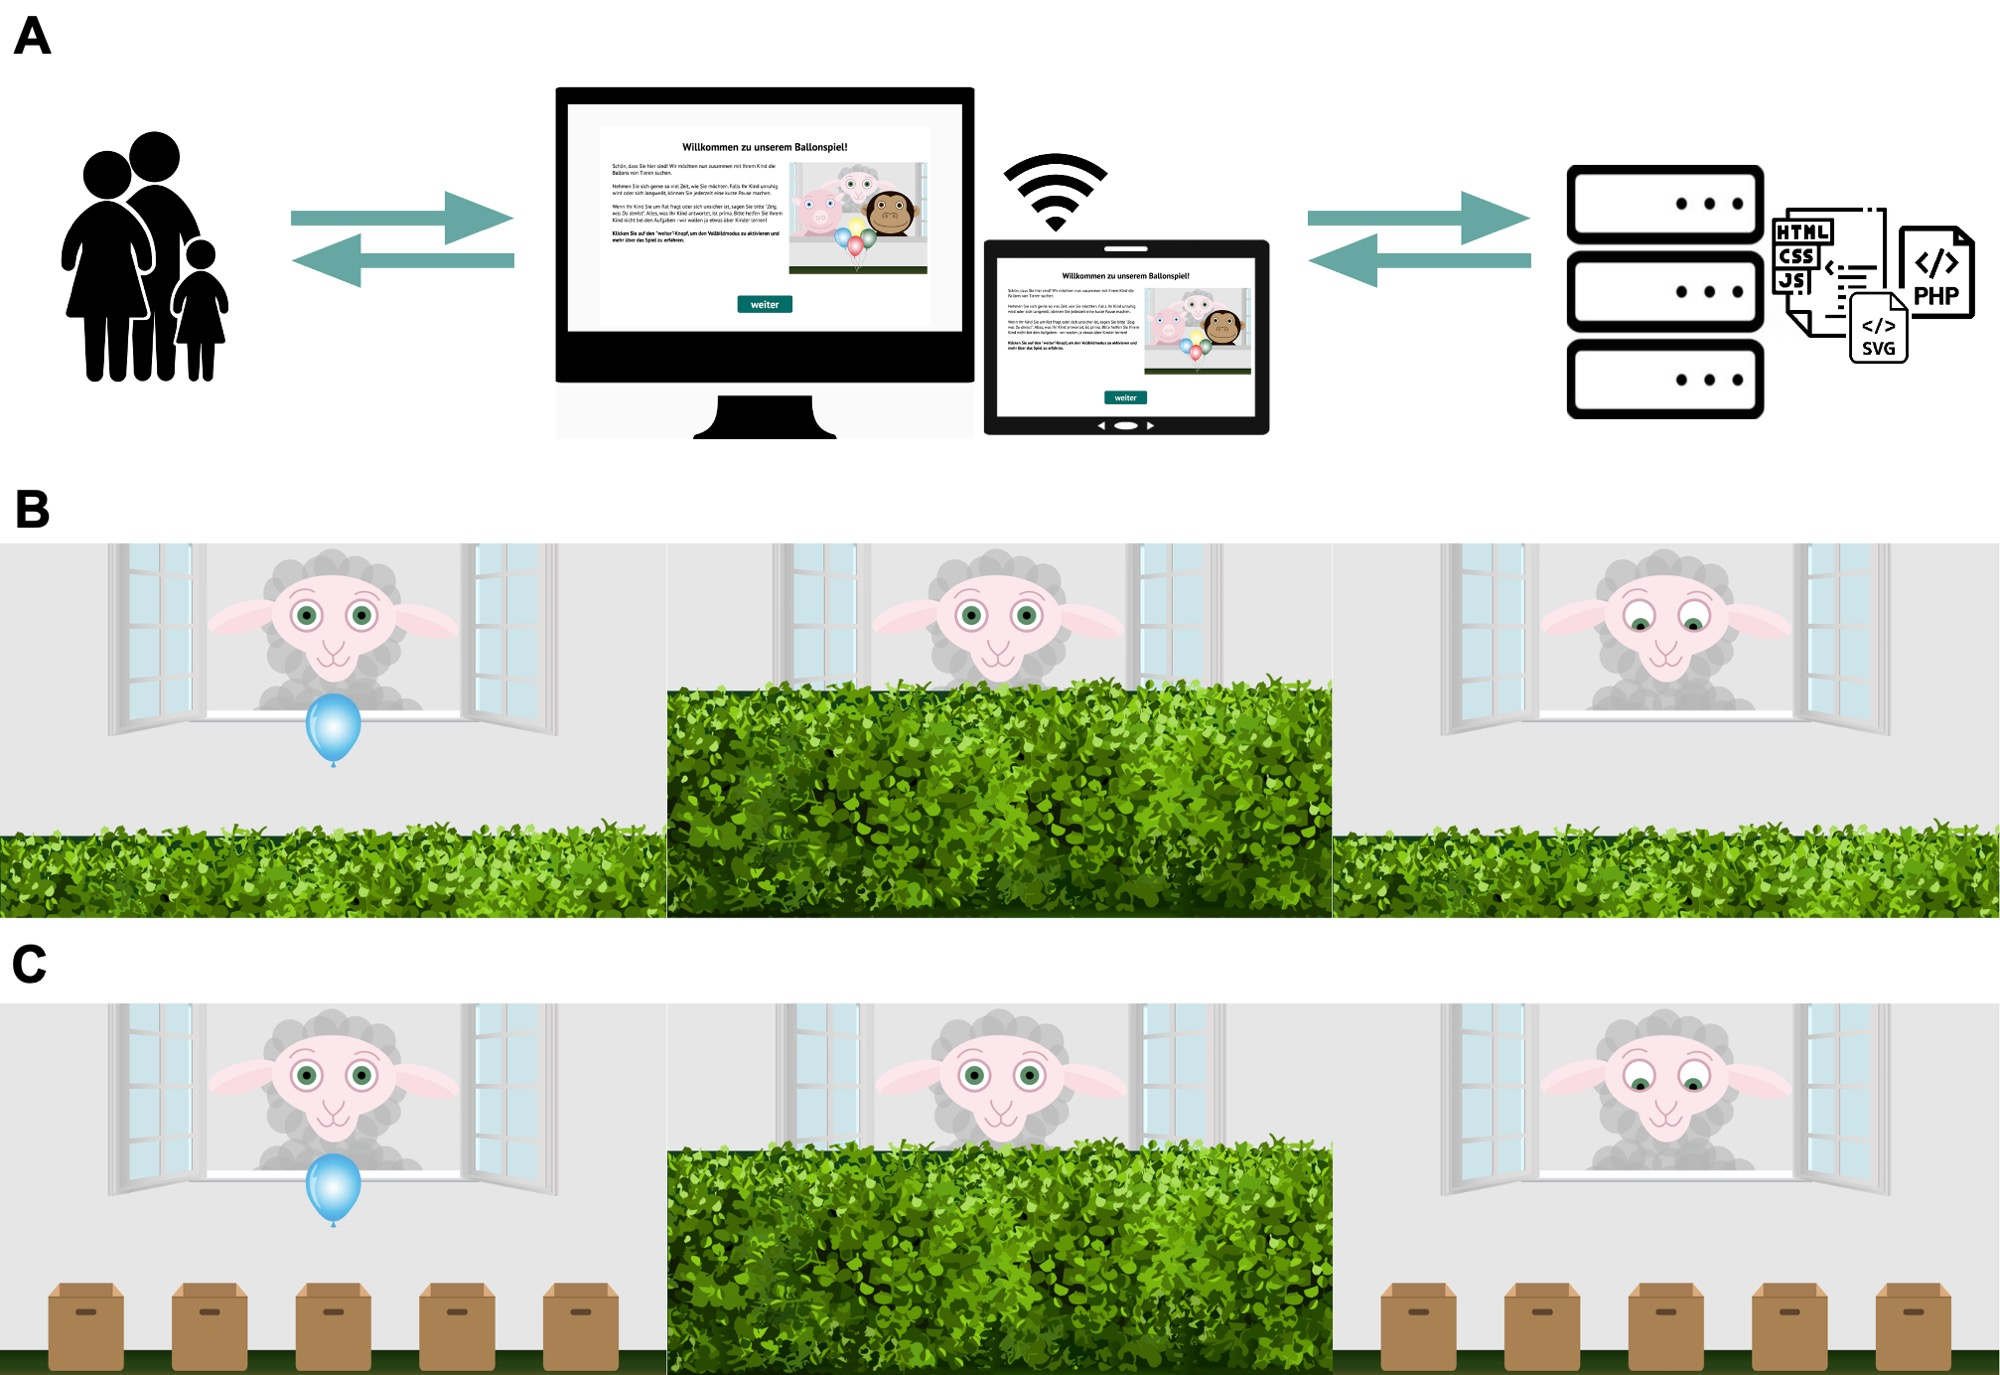
\includegraphics[width=1\linewidth]{../figures/gafo_procedure} 

}

\caption{\textbf{Study setup}.
(a) Infrastructure for online testing. (i) Subjects aged 3 -- 99+ can participate. Data collection can take place anywhere: at home, in kindergartens or research institutes. (ii) The task is presented as a website that works across devices. (iii) The scripts for the website and the recorded data are stored on secure local servers.
(b) Continuous \emph{hedge} version of the balloon finding task. (i) The agent stands in a window with the target in front of them. (ii) A hedge grows and covers the target. (iii) The target falls to a random location on the ground. The agent's eyes track the movement of the target.
(c) Discrete \emph{box} version of the balloon finding task. Number of boxes (min. 1; max. 8) as potential hiding locations can be set individually.}\label{fig:fig1}
\end{figure}

\hypertarget{randomization}{%
\subsection{Randomization}\label{randomization}}

All agents and target colors appear equally often and are not repeated in more than two consecutive trials. The randomization of the target end location depends on the study version. In the \emph{hedge} version, the full width of the screen is divided into ten bins. Exact coordinates within each bin are then randomly generated. In the \emph{box} version, the target randomly lands in one of the boxes. As with agent and color choice, each bin/box occurs equally often and can only occur twice in a row.

\hypertarget{implementation}{%
\subsection{Implementation}\label{implementation}}

Our balloon finding task is presented as an interactive web-app. The task is portable across devices and web browsers and does not require any installation. A great advantage of online testing is that our testing procedure is standardized across participants. By using pre-recorded study instructions, no interaction with the experimenter is necessary during the study. The code is open-source (\url{https://github.com/ccp-eva/gafo-demo}) and a live demo version can be found under: \url{https://ccp-odc.eva.mpg.de/gafo-demo/}.
The web-app was programmed in JavaScript (ECMAScript 2015, i.e., ES6), HTML5, CSS and PHP.
We utilized the zero configuration bundler Parcel to enable a live server for debugging, easy imports and minified scripts in order to save data storage.
For stimulus presentation, a scalable vector graphic (SVG) composition was parsed. This way, the composition scales according to the user's view port without loss of quality, while keeping the aspect ratio and relative object positions constant.
Furthermore, SVGs allow us to define all composite parts of the scene (e.g., pupil of the agent) individually. This is needed for precisely calculating exact pupil and target locations and sizes. Additionally, it makes it easy to adjust the stimuli and, for example, add another agent to the scene.
The GreenSock Animation Platform (GSAP; Greensock (2022)) library was used to animate the movement of single SVG elements.
We use URL parameters to capture the participant's ID, language and study version.
The web-app generates two file types: (1) a text file (.json) containing meta-data, trial specifications and participants' click responses, and (2) a video file (.webm) of the participant's webcam recording.
For our samples described in this paper, we deployed the web-app on servers located in Leipzig, Germany. Data got automatically collected and safely stored on these in-house servers. If no internet connection or server is available, researchers could download a local version of the experiment which stores the generated data automatically on the used device. For child samples, we upload safety copies of the already collected responses after the fourth test trial. In cases where children want to stop participation earlier, no responses get lost.

\hypertarget{data-processing}{%
\subsection{Data processing}\label{data-processing}}

We used R version 4.1.3 (2022-03-10) (R Core Team, 2022), and the packages \emph{splithalfr} (Pronk, Molenaar, Wiers, \& Murre, 2021) and \emph{brms} (Bürkner, 2017, 2018) for all our analyses. Regression models were fitted as Bayesian generalized linear mixed models (GLMMs) with default priors for all analyses.
All test trials without voice over description are included in our analyses.

\hypertarget{does-the-balloon-finding-task-induce-variation}{%
\section{Does the balloon finding task induce variation?}\label{does-the-balloon-finding-task-induce-variation}}

Our first aim was to assess whether our balloon finding task induces interindividual variation in a child and adult sample. Furthermore, we were interested in how the data collection mode influences responses. To analyze how the in-person collected data compares to data that gets collected in a online without supervision, we collected a remote child and adult sample.

The pre-registrations can be found here: \url{https://osf.io/snju6} (child sample) and here: \url{https://osf.io/r3bhn} (adult sample). Participants were equally distributed across the two study versions. The study was approved by an internal ethics committee at the Max Planck Institute for Evolutionary Anthropology. Data was collected between May and October 2021.

\hypertarget{participants}{%
\subsection{Participants}\label{participants}}

We collected data from an in-person child sample, a remote child sample, and a remote adult sample.
In-person testing with children took place in kindergartens in Leipzig and surroundings that cooperate with the Max Planck Institute for Evolutionary Anthropology. The in-person child sample consisted of
120 children, including
40 3-year-olds
(mean = 41.45 months,
SD = 3.85,
range = 36
- 47,
22 girls),
40 4-year-olds
(mean = 54.60 months,
SD = 3.10,
range = 48
- 59,
19 girls),
and 40 5-year-olds
(mean = 66.95 months,
SD = 3.39,
range = 60
- 71,
22 girls).

For our remote child sample, we recruited families on a voluntary basis via email from the institute's internal database. Our remote child sample included 147 children, including
45 3-year-olds
(mean = 42.62 months,
SD = 3.35,
range = 36
- 47,
14 girls),
47 4-year-olds
(mean = 52.64 months,
SD = 3.40,
range = 48
- 59,
25 girls),
and 55 5-year-olds
(mean = 65.11 months,
SD = 3.77,
range = 60
- 71,
27 girls). Children in our sample grow up in an industrialized, urban Central-European context. Information on socioeconomic status was not formally recorded, although the majority of families come from mixed, mainly mid to high socioeconomic backgrounds with high levels of parental education.

In addition, we recruited a remote adult sample by advertising the study on \emph{Prolific}. \emph{Prolific} is an online participant recruitment service from the University of Oxford with a predominantly European and US-american subject pool. Participants consisted of 100 English-speakers with an average age of 31.34 years (SD = 10.77, range = 18 - 63, 64 females).
For completing the study, subjects were payed above the fixed minimum wage (in average £10.00 per hour). \emph{Prolific} distributed our study link to potential participants, while the hosting of the online study was done by local servers in the Max Planck Institute for Evolutionary Anthropology, Leipzig, Germany.

\hypertarget{procedure}{%
\subsection{Procedure}\label{procedure}}

Children in our in-person sample were tested on a tablet in a quiet room in their daycare center. An experimenter accompanied the child and helped them navigate through the online study.
Children in the remote sample received a personalized link to the study websites and families could participate at any time or location they wanted. In the beginning of the online study, families were invited to enter our ``virtual institute'' and were welcomed by an introductory video of the study leader, shortly describing the research background and further procedure. Then, caregivers were informed about data security and were asked for their informed consent. They were asked to enable the sound and seat their child centrally in front of their device. Before the study started, families were instructed how to setup their webcam and enable the recording permissions. We stressed that caregivers should not help their children. Study participation was video recorded whenever possible in order to ensure that the answers were generated by the children themselves.
Depending on the participant's device, the website automatically presented the hedge or box version of the study. For families that used a tablet with touchscreen, the hedge version was shown. Here, children could directly click on the touchscreen themselves to indicate where the target is. For families that used a computer without touchscreen, the website presented the box version of the task. We assumed that younger children in our sample would not be acquainted with the usage of a computer mouse. Therefore, we asked children to point to the screen, while caregivers were asked to act as the ``digital finger'' of their children and click on the indicated box.

Our adult sample participated remotely without supervision.

All participants received 15 test trials that were displayed as described above. In the box version, we decided to adjust the task difficulty according to the sample: children were presented with five boxes while adults were presented with eight boxes as possible target locations.

\hypertarget{results}{%
\subsection{Results}\label{results}}










\begin{figure}

{\centering 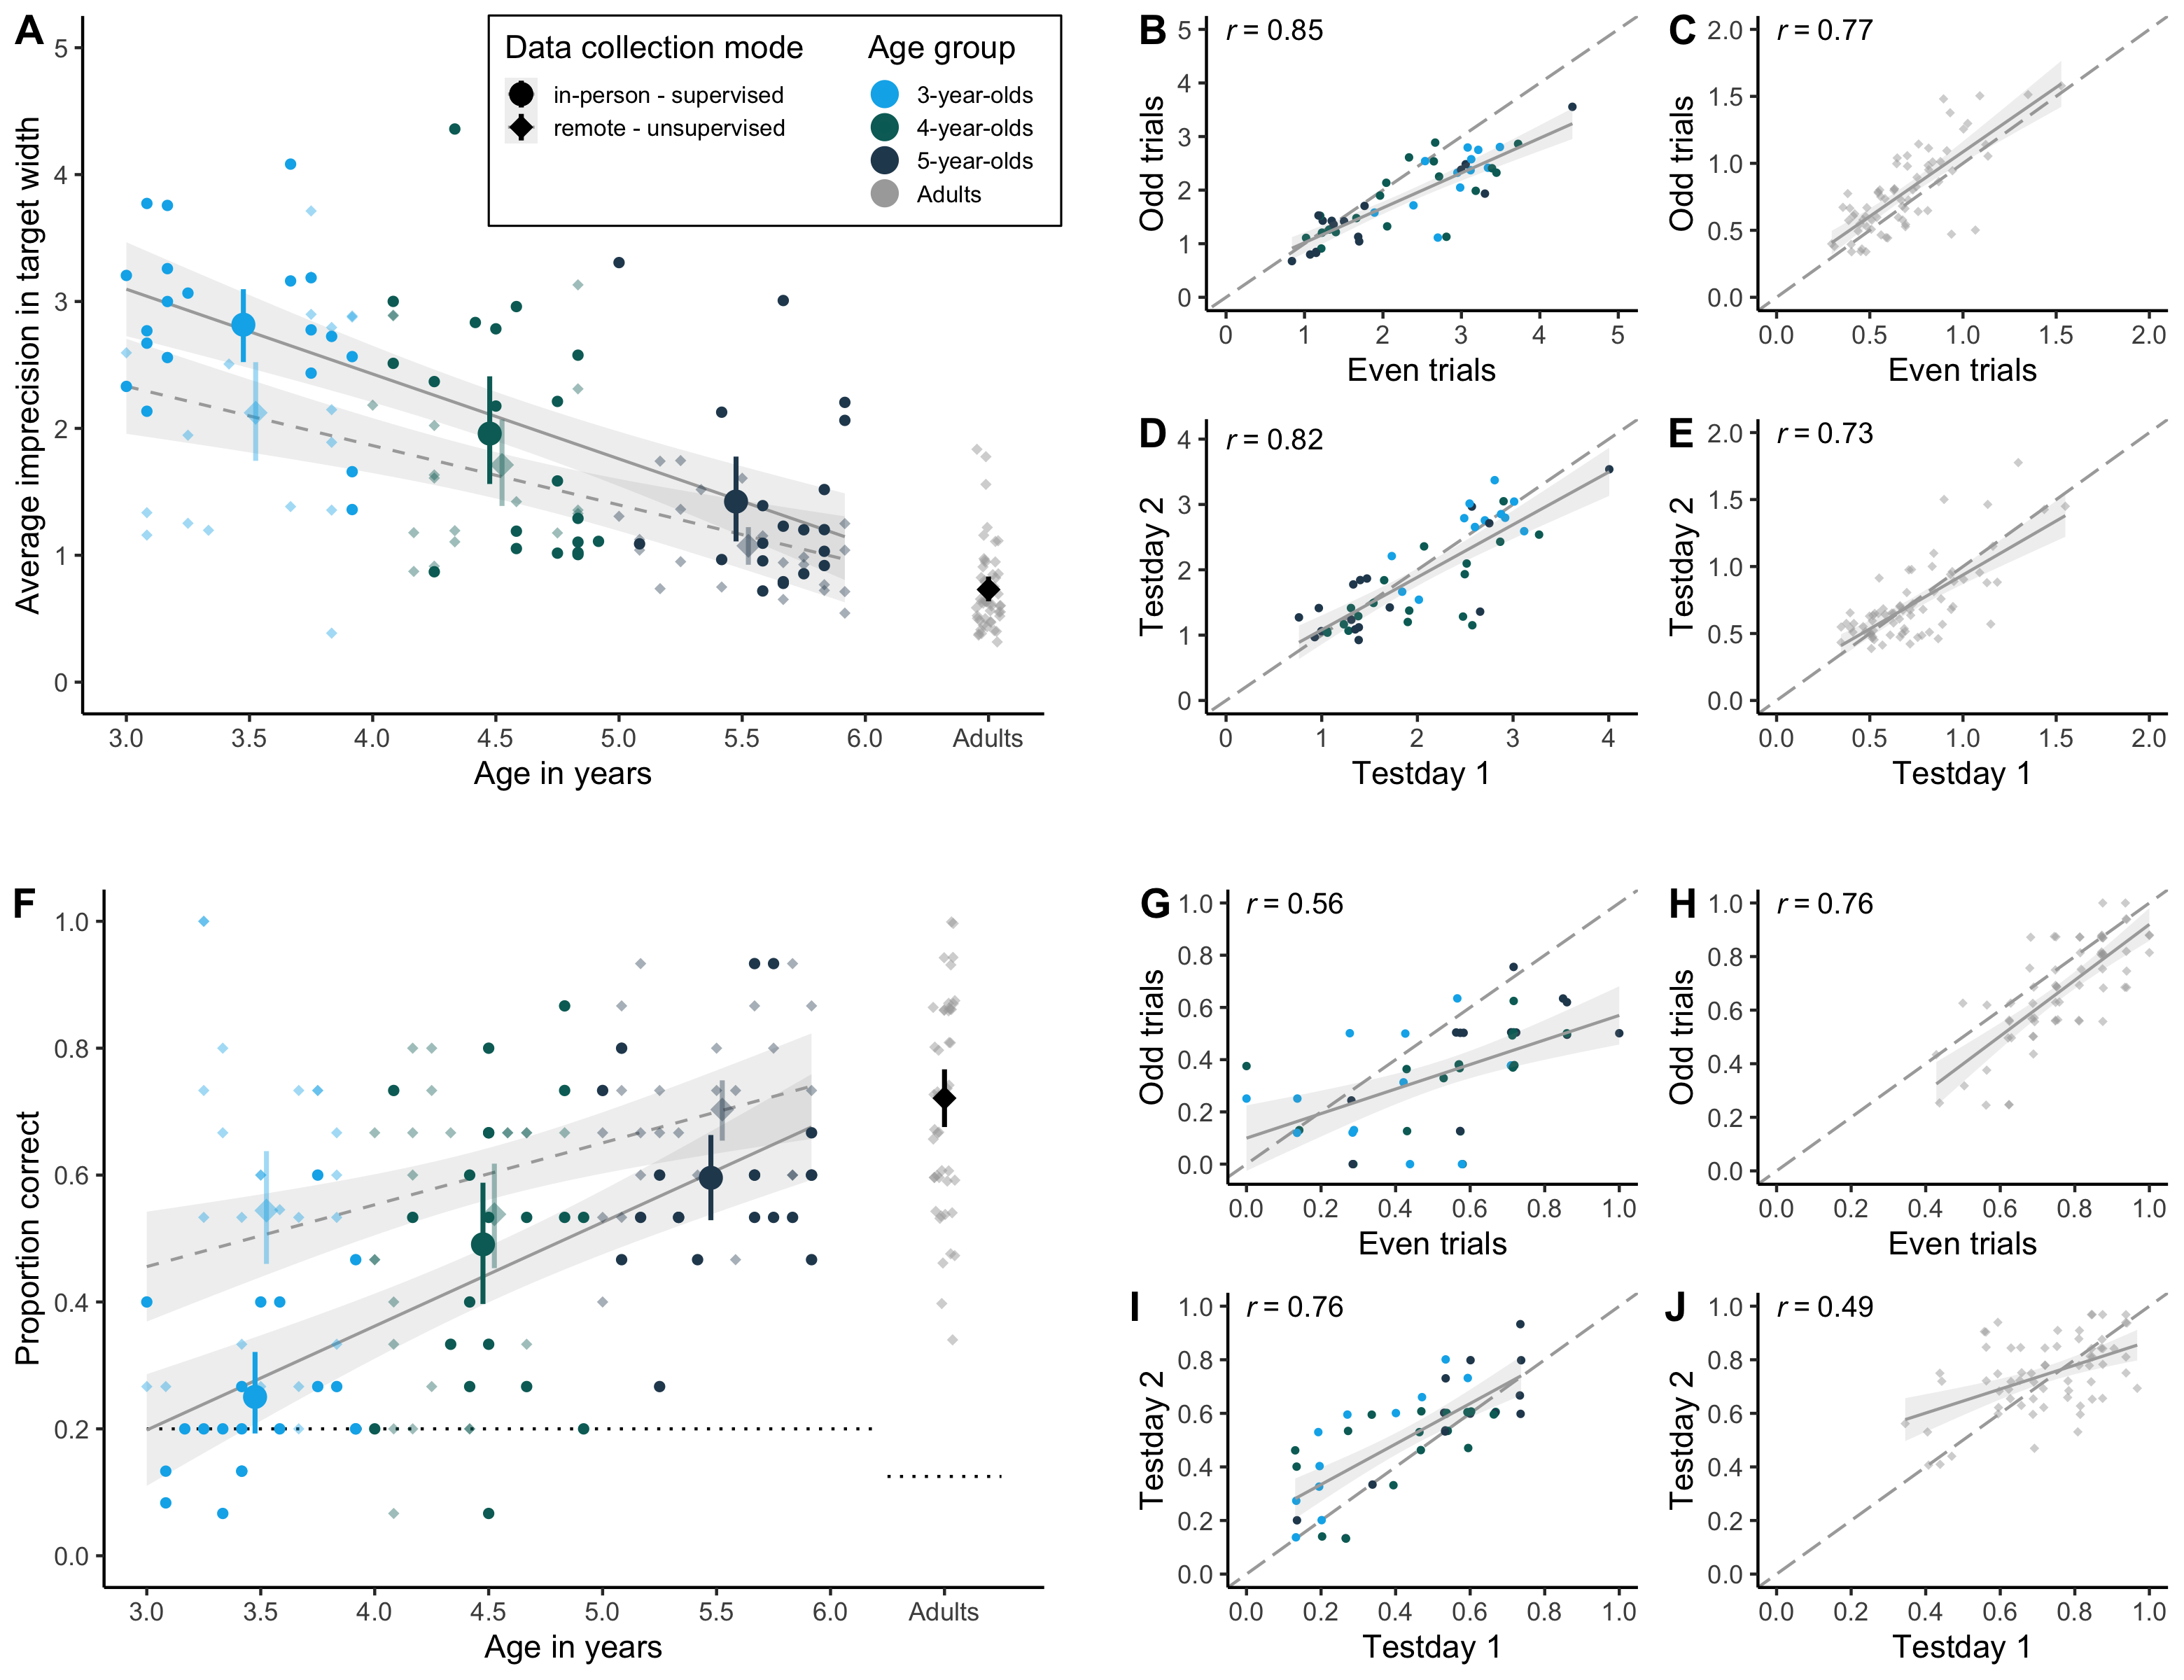
\includegraphics[width=1\linewidth]{../figures/gafo_results} 

}

\caption{\textbf{Measuring interindividual variation}.
(a) Developmental trajectory in continuous \emph{hedge} version. Performance is measured as average imprecision, i.e., the absolute distance between the target's center and the participant's click. The unit of imprecision is counted in the width of the target, i.e., a participant with an imprecision of 1 clicked in average one target width to the left or right of the true target center.
(b) Internal consistency (odd-even split) in hedge child sample. (c) Internal consistency in hedge adult sample. (d) Test-retest reliability in hedge child sample. (e) Test-retest reliability in hedge adult sample.
(f) Developmental trajectory in discrete \emph{box} version. Performance is measured as the proportion of correct responses, i.e., how many times the participant clicked on the box that actually contained the target. Dotted black line shows level of performance expected by chance (for child sample 20\%, i.e., 1 out of 5 boxes; for adult sample 12.5\%, i.e., 1 out of 8 boxes).
(g) Internal consistency (odd-even split) in box child sample. (h) Internal consistency in box adult sample. (i) Test-retest reliability in box child sample. (j) Test-retest reliability in box adult sample.
Regression lines with 95\% CI show product-moment-correlations with Pearson's correlation coefficient r.
Large data points with 95\% CI (based on non-parametric bootstrap) represent performance means by age group (binned by year).
Small data points show the mean performance for each subject. Shape of data points represents data collection mode: opaque round circles with stand for in-person supervised data collection, translucent diamonds stand for remote unsupervised data collection. Color of data points represent each age group (binned by year).}\label{fig:fig2}
\end{figure}

We captured a developmental trajectory of gaze cue understanding: with increasing age, participants got more and more accurate in locating the target. In the hedge version, children's click imprecision droped with age, while, congruently, the proportion of correct responses increased in the box version (see Figure 2 A and F). By the end of their sixth year of life, children came close to the adult's proficiency level. We found interindividual variation across study versions and age groups: some three-year-olds were more precise in their responses than some five-year-olds.

As Figure 2 A and F show, our remotely collected data resembled the data from the kindergarten sample.
To quantify the effect sizes, we formulated a Bayesian generalized linear mixed model with age (in months, z-transformed) and data collection mode (with in-person supervised data collection as the reference category), and target position and subject ID as random effects. In the hedge version, we found an estimate of age of -0.33 (95\% CI {[}-0.42; -0.23{]}) and an estimate of data collection mode of -0.32 (95\% CI {[}-0.50; -0.14{]}).
In the box version, the estimate of age was 0.64 (95\% CI {[}0.41; 0.88{]}) and the estimate of data collection mode was 1.16 (95\% CI {[}0.73; 1.61{]}). Note that the effect of data collection appears to be present, but confidence intervals are wide.

Our GLMM analysis, therefore, corroborated the effects of age and data collection mode that we already identified by visual inspection.
We found evidence that responses of children participating remotely were slightly more precise. This difference was mainly driven by the younger participants and especially prominent in the box version of the task. It is conceivable that caregivers were especially prone to influence the behavior of younger children. In the box version, caregivers might have had more opportunities to interfere since they carried out the clicking for their children.\footnote{In an exploratory analysis, we coded parental behavior and environmental factors during remote unsupervised testing. Due to the incredible time consuming nature of hand coding videos frame by frame, we focused on the subsample with the greatest performance difference between data collection modes: the three-year-olds in the box version of the task (n = 16). We reasoned that if parental interference cannot explain the greatest performance difference in our sample, the effects would be negligible in the remaining sample.
  A trial was defined as the time between two eye blinking sounds. We transcribed all utterances by parents and children and counted the words uttered by each. We then classified the utterances into several categories: question asked by child, repeated testquestion by caregiver, hints towards agents (how many times the caregivers guided the child's attention to the agent), hints towards eyes (how many times the caregivers guided the child's attention to the agent's eyes), verification of choice (how many times the caregiver questioned or double checked the child's response), mentioning of screen (how many times the caregiver verbally guided the child's attention to the screen), pointing to screen (how many times the caregiver pointed towards the screen), positive \& negative feedback, motivational statements, and incomprehensible utterances.
  In addition, we coded how many adults and children were present, whether a response click was obviously conducted by the caregiver themselves, and whether children took a break during the trial.
  We ran exploratory analyses . Remaining variables that we coded for were not included since there was not enough variation and/or occurrences in our sample. Our null model explained the the response behavior by age, while including random effects for subject and target position. We compared this null model to models including the number of words utterred by the caregiver, number of repeated testquestions, verification of choice, or hints towards eyes. Furthermore, we calculated an parental interference index by summing up number of repeated testquestions, verification of choice, and hints towards eyes, with the sign matching the variable's direction of effect.
  On the trial level, the model including the verification of choice as a main effect won: here, the less the caregivers asked for children's responses again, the more likely children clicked on the correct box. On a subject level, the effect reversed - possibly due to greatest learning effects for the children that were most likely to click incorrectly in the beginning and then receiving most parental comments. Additionally, number of repeated testquestions displayed a negative estimate on the subject level: the more caregivers asked again where the target landed, the more likely children were to respond to the incorrect box. {[}TODO:{]} In all cases, however, standard errors of the WAIC score differences where greater than the ELPD difference scores themselves. Similarly, 95\% CI of the model estimates included zero and were rather wide. Therefore, we conclude that no stable effect of parental interference could be confirmed in this exploratory analysis.}

\hypertarget{discussion}{%
\subsection{Discussion}\label{discussion}}

Study 1 showed that our newly implemented balloon finding task can be used to study gaze cue understanding in both children and adults. With increasing age, participants got more and more precise in locating the target. We found interindividual variation across all age groups. Furthermore, we found a comparable developmental trajectory for an unsupervised remote child sample. This underlines how flexibly our new task can be used.

\hypertarget{can-we-capture-variation-reliably}{%
\section{Can we capture variation reliably?}\label{can-we-capture-variation-reliably}}

As a next step we aimed at investigating whether the variation that we captured with our balloon finding task is reliable. For this aim, we assessed the internal consistency, as calculated by splithalf reliability, and the test-retest reliability. The pre-registrations can be found here: \url{https://osf.io/xqm73} (child sample) and here: \url{https://osf.io/nu62m} (adult sample). Participants were equally distributed across the two study versions. The study was approved by an internal ethics committee at the Max Planck Institute for Evolutionary Anthropology. Data was collected between July 2021 and April 2022.

\hypertarget{participants-1}{%
\subsection{Participants}\label{participants-1}}

For our child sample, we again went to kindergartens in Leipzig and surroundings.
The child sample consisted of
93 children, including
24 3-year-olds
(mean = 42.49 months,
SD = 2.99,
range = 38
- 47,
13 girls),
38 4-year-olds
(mean = 53.77 months,
SD = 3.16,
range = 48
- 59,
19 girls),
and 31 5-year-olds
(mean = 66 months,
SD = 3.42,
range = 61
- 71,
17 girls).

The adult sample was again recruited over \emph{Prolific} and consisted of 136 English-speakers with an average age of 25.74 years (SD = 8.11, range = 18 - 71, 87 females).

\hypertarget{procedure-1}{%
\subsection{Procedure}\label{procedure-1}}

We applied the same procedure as in the first study, with the following differences. Participants completed the study twice, with a delay of 14 ± 3 days.
The target locations as well as the succession of animals and target colors was randomized once and then held constant across participants.
The child sample received 15 test trials. In the hedge version, each bin occurred once, making up ten of the test trials. For the remaining five test trials, we repeated one out of two adjacent bins (i.e., randomly chose between bin 1 \& 2, bin 3 \& 4, etc). In the box version, we ensured that each of the five boxes occurred exactly three times. For the remaining training trials, we repeated a fixed order of four random bins/boxes.
Adults in the hedge version received 30 test trials, each of the ten bin occurring exactly three times. Adults in the box version received 32 test trials with each of the eight boxes occurring exactly four times.

\hypertarget{results-1}{%
\subsection{Results}\label{results-1}}

As a first step for estimating the reliability of our task, we focused on the internal consistency by calculating splithalf reliability coefficients. Trials were split into two equally big parts and the performance scores per part were correlated against each other. We used the raw performance per subject of the first test day. Traditional odd-even splits on our data and the corresponding \emph{Pearson} correlation coefficients are shown in Figure 2 B, C, G and H.

As a recent paper by Pronk et al. (2021) suggested, there are various, more sophisticated split-half methods that differ in how the trials are split into parts and whether they are combined with stratification by task design.
To compare our traditional approach of a simple odd-even split, we additionally calculated reliability estimates using first-second, odd-even, permutated, and Monte Carlo splits without and with stratification by target position. First-second and odd-even splits belong to single sample methods, since each participant has a single pair of performance scores, while permutated (without replacement) and Monte Carlo (with replacement) splits make use of resampling.
In the hedge version, reliability coefficients ranged from 0.57 to 0.87. In the box version, reliability coefficients ranged from 0.43 to 0.76.
Similarly to the results of Pronk et al. (2021), we found that more robust splitting methods that are less prone to task design or time confounds yielded higher reliability coefficients. In the majority of cases, stratifying by target position lead to similar or even higher estimates compared to no stratification. As might be expected, we found higher coefficients for the samples with higher variation, i.e., for our continuous hedge version of the task.




\begin{figure}

{\centering 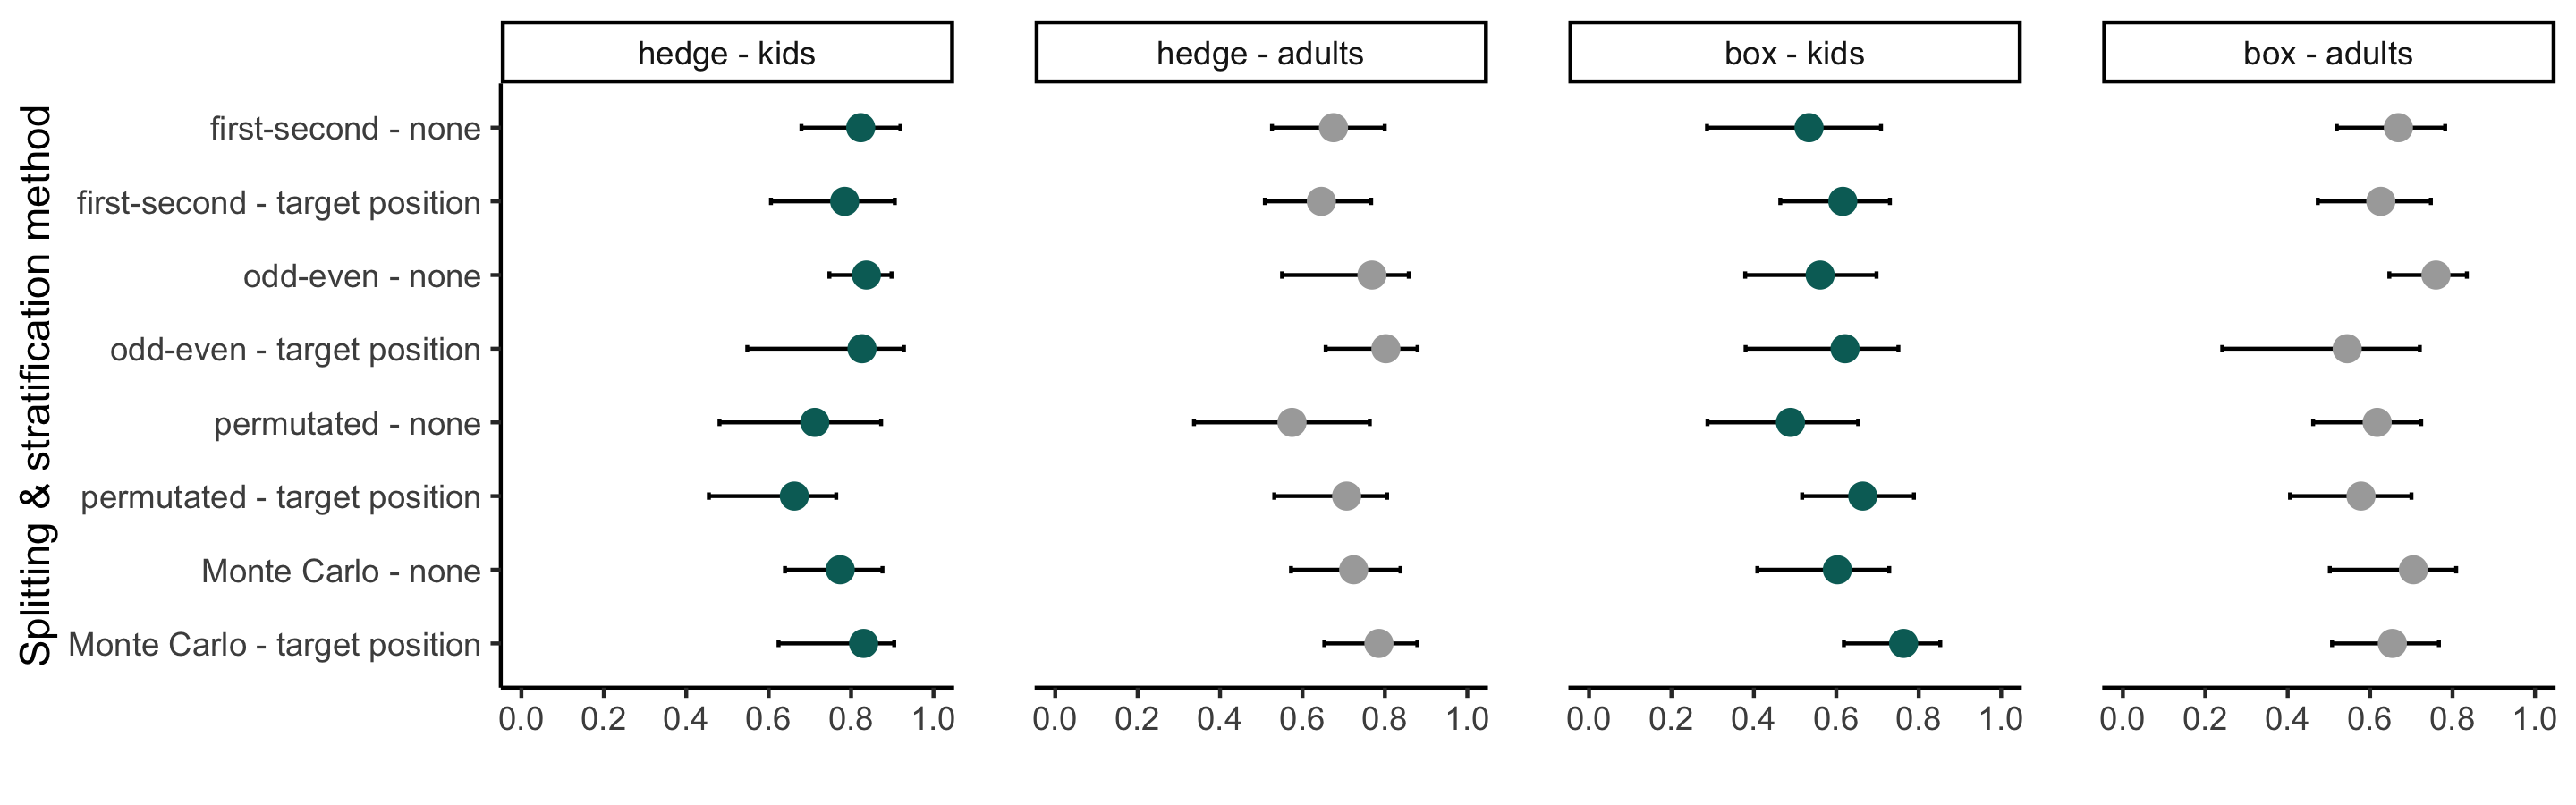
\includegraphics[width=1\linewidth]{../figures/gafo_splithalf} 

}

\caption{\textbf{Internal Consisteny}.
Reliability coefficients per splitting method, stratification level, study version and age group. Error bars show the 95\% confidence intervals of the coefficient estimates.}\label{fig:fig3}
\end{figure}

\hypertarget{discussion-1}{%
\subsection{Discussion}\label{discussion-1}}

Our results indicated that the measured variation was systematic. These results hold for both the continuous hedge version as well as the discrete box version of the task.

\hypertarget{exploring-the-external-validity-of-our-task}{%
\section{Exploring the external validity of our task}\label{exploring-the-external-validity-of-our-task}}

Our third aim was to assess whether the captured individual variation in gaze cue understanding relates to factors in children's real live social surroundings.

\hypertarget{participants-2}{%
\subsection{Participants}\label{participants-2}}

For this exploratory analysis, we included all children of the aforementioned samples where families filled out a short demographic questionnaire. This subsample consisted of
130 children, including
39 3-year-olds
(mean = 43.02 months,
SD = 3.20,
range = 37
- 47,
20 girls),
44 4-year-olds
(mean = 54.43 months,
SD = 2.77,
range = 48
- 59,
26 girls),
and 47 5-year-olds
(mean = 66.13 months,
SD = 3.55,
range = 60
- 71,
23 girls).

\hypertarget{procedure-2}{%
\subsection{Procedure}\label{procedure-2}}

Families of our kindergarten and online child sample were asked to fill out a brief demographic questionnaire (print out / online questionnaire). We asked for (1) the total number of household members, (2) the number of children, (3) age of the other children, (4) whether the child was in day care, and if yes, (5) since when and (6) for how long on an average day.

\hypertarget{results-2}{%
\subsection{Results}\label{results-2}}

\begin{itemize}
\tightlist
\item
  peer exposure (hedge \& box combined?)
\end{itemize}

\hypertarget{discussion-2}{%
\section{Discussion}\label{discussion-2}}

\hypertarget{limitations}{%
\subsection{Limitations}\label{limitations}}

\hypertarget{future-development-extending-the-task}{%
\subsection{Future development / extending the task}\label{future-development-extending-the-task}}

\hypertarget{conclusion}{%
\section{Conclusion}\label{conclusion}}

\hypertarget{declarations}{%
\section{Declarations}\label{declarations}}

\hypertarget{open-practices-statement}{%
\subsection{Open practices statement}\label{open-practices-statement}}

The web application (\url{https://ccp-odc.eva.mpg.de/gafo-demo/}) described here is open source (\url{https://github.com/ccp-eva/gafo-demo}).
The datasets generated during and/or analysed during the current study are available in the {[}gazecues-methods{]} repository, (\url{https://github.com/jprein/gazecues-methods}). All experiments were preregistered (\url{https://osf.io/zjhsc/}).

\hypertarget{funding}{%
\subsection{Funding}\label{funding}}

This study was funded by the Max Planck Society for the Advancement of Science, a noncommercial, publicly financed scientific organization (no grant number). We thank all the children and parents who participated in the study.

\hypertarget{conflicts-of-interest}{%
\subsection{Conflicts of interest}\label{conflicts-of-interest}}

The authors declare that they have no conflict of interest.

\hypertarget{ethics-approval}{%
\subsection{Ethics approval}\label{ethics-approval}}

\hypertarget{consent-to-participate}{%
\subsection{Consent to participate}\label{consent-to-participate}}

Informed consent was obtained from all individual participants included in the study or their legal guardians.

\hypertarget{consent-for-publication}{%
\subsection{Consent for publication}\label{consent-for-publication}}

\hypertarget{open-access}{%
\subsection{Open access}\label{open-access}}

\hypertarget{authors-contributions}{%
\subsection{Authors' contributions}\label{authors-contributions}}

optional: please review the submission guidelines from the journal whether statements are mandatory

\newpage

\hypertarget{references}{%
\section{References}\label{references}}

\begingroup
\setlength{\parindent}{-0.5in}
\setlength{\leftskip}{0.5in}

\hypertarget{refs}{}
\begin{CSLReferences}{1}{0}
\leavevmode\vadjust pre{\hypertarget{ref-burkner2017brms}{}}%
Bürkner, P.-C. (2017). Brms: {An R Package} for {Bayesian Multilevel Models Using Stan}. \emph{Journal of Statistical Software}, \emph{80}(1). \url{https://doi.org/10.18637/jss.v080.i01}

\leavevmode\vadjust pre{\hypertarget{ref-burkner2018advanced}{}}%
Bürkner, P.-C. (2018). Advanced {Bayesian Multilevel Modeling} with the {R Package} brms. \emph{The R Journal}, \emph{10}(1), 395. \url{https://doi.org/10.32614/RJ-2018-017}

\leavevmode\vadjust pre{\hypertarget{ref-greensock2022gsap}{}}%
Greensock. (2022). \emph{{GSAP} ({GreenSock Animation Platform})}.

\leavevmode\vadjust pre{\hypertarget{ref-pronk2021methods}{}}%
Pronk, T., Molenaar, D., Wiers, R. W., \& Murre, J. (2021). Methods to split cognitive task data for estimating split-half reliability: {A} comprehensive review and systematic assessment. \emph{Psychonomic Bulletin \& Review}. \url{https://doi.org/10.3758/s13423-021-01948-3}

\leavevmode\vadjust pre{\hypertarget{ref-rcoreteam2022language}{}}%
R Core Team. (2022). \emph{R: {A} language and environment for statistical computing} {[}Manual{]}. {Vienna, Austria}: {R Foundation for Statistical Computing}.

\end{CSLReferences}

\endgroup

\newpage

\hypertarget{supplements}{%
\section{Supplements}\label{supplements}}

\hypertarget{adult-sample}{%
\subsection{Adult sample}\label{adult-sample}}

\hypertarget{recruitment}{%
\subsubsection{Recruitment}\label{recruitment}}

We recruited participants using the online participant recruitment service \emph{Prolific} from the University of Oxford. \emph{Prolific}'s subject pool consists of a mostly European and US-american sample although subjects from all over the world are included. The recruitment platform realises ethical payment of participants, which requires researchers to pay participants a fixed minimum wage of £5.00 (around US\$6.50 or €6.00) per hour. We decided to pay all participants the same fixed fee which was in relation to the estimated average time taken to complete the task.
\emph{Prolific} distributed our study link to potential participants, while the hosting of the online study was done by local servers in the Max Planck Institute for Evolutionary Anthropology, Leipzig. Therefore, study data was saved only on our internal servers, while \emph{Prolific} provided demographic information of the participants.
Participants' \emph{Prolific} ID was forwarded to our study website using URL parameters. This way, we could match participant demographic data to our study data. The same technique was used to confirm study completion: we redirected participants from our study website back to the \emph{Prolific} website using URL parameters.
We used \emph{Prolific}'s inbuilt prescreening filter to include only participants who were fluent in English and could therefore properly understand our written and oral study instructions.

\hypertarget{study-1---validation-hedge-version}{%
\subsubsection{Study 1 - Validation hedge version}\label{study-1---validation-hedge-version}}

The aim of Study 1 was to validate the hedge version of our balloon finding task. The pre-registration can be found here: \url{https://osf.io/r3bhn}. We recruited participants online by advertising the study on \emph{Prolific}.

50 adults participated in the study. One additional subject returned their submission, i.e., decided to leave the study early or withdrew their submission after study completion. Data collection took place in May 2021.
Participants were compensated with £1.25 for completing the study. We estimated an average completion time of 6 minutes, resulting in an estimated hourly rate of £10.00. In average, participants took 05:56min to complete the study.
Participants were required to complete the study on a tablet or desktop. Participation on mobile devices was disabled since the display would be too small and would harm click precision. It was indicated that the study required audio sound.

We stored \emph{Prolific}'s internal demographic information, while not asking for additional personal information.

\hypertarget{study-2---validation-box-version}{%
\subsubsection{Study 2 - Validation box version}\label{study-2---validation-box-version}}

As in study 1, we recruited participants on \emph{Prolific}, and employed the same methodology. However, this time we focussed on validating the box version of the task in an adult sample. Participants were presented with eight boxes in which the target could land.
50 adults participated in the study. One additional subject returned their submission, i.e., decided to leave the study early or withdrew their submission after study completion. Data collection took place in June 2021.
Participants were compensated with £1.00 for completing the study. We estimated an average completion time of 6 minutes, resulting in an estimated hourly rate of £10.00. In average, participants took 04:43min to complete the study.

\hypertarget{study-3---reliability-hedge-version}{%
\subsubsection{Study 3 - Reliability hedge version}\label{study-3---reliability-hedge-version}}

In study 3 and 4, we assessed the test-retest reliability of our balloon-finding task in an adult sample. The pre-registration can be found here: \url{https://osf.io/nu62m}. We tested the same participants twice with a delay of two weeks. The testing conditions were as specified in Study 1 and 2. However, the target locations as well as the succession of animals and target colors was randomized once. Each participant then received the same fixed randomized order of target location, animal, and target color. Participants received 30 test trials without voice-over description, so that each of the ten bins occurred exactly three times.

In addition to the beforementioned prescreening settings, we used a whitelist. \emph{Prolific} has a so-called \emph{custom allowlist prescreening filter} where one can enter the \emph{Prolific} IDs of participants who completed a previous study. Only these subjects are then invited to participate in a study. This way, repeated measurements can be implemented, collecting data from the same subjects at different points in time.

In a first round, 60 participants took part on the first testday. Additional two subjects returned their submission, i.e., decided to leave the study early or withdrew their submission after study completion. One additional participant timed out, i.e., did not finish the survey within the allowed maximum time. The maximum time is calculated by \emph{Prolific}, based on the estimated average completion time. For this study, the maximum time amounted to 41 minutes. For the first testday, participants were compensated with £1.25. We estimated an average completion time of 9 minutes, resulting in an estimated hourly rate of £8.33. In average, participants took 07:11min to complete the first part.

Of the 60 participants that completed testday 1, 41 subjects finished testday 2. One additional participant timed out, i.e., did not finish the survey within the allowed maximum time. Participants were compensated with £1.50 for completing the second part of the study. We estimated an average completion time of 9 minutes, resulting in an estimated hourly rate of £10. In average, participants took 06:36min to complete the second part of the study.

Since we aimed for a minimum sample size of 60 subjects participating on both testdays, we reran the first testday with additional 50 participants. Additional seven subjects returned their submission, i.e., decided to leave the study early or withdrew their submission after study completion. Two additional participants timed out, i.e., did not finish the survey within the allowed maximum time. Again, participants were compensated with £1.25 for completing the first part of the study (estimated average completion time 9 minutes, estimated hourly rate of £8.33). In average, participants took 06:51min to complete the first part.

Of the additional 50 participants that completed testday 1, 29 subjects finished testday 2. Again, participants were compensated with £1.50 for completing the second part of the study (estimated average completion time 9 minutes, estimated hourly rate of £10). In average, participants took 06:26min to complete the second part of the study.

\hypertarget{study-4---reliability-box-version}{%
\subsubsection{Study 4 - Reliability box version}\label{study-4---reliability-box-version}}

As in study 3, we recruited participants on \emph{Prolific}, and employed the same methodology. However, this time participants were presented with the box version of the task. Participants received 32 test trials without voice-over description, so that each of the eight boxes occurred exactly four times. As in study 2, we employed eight boxes in which the target could land.

In a first round, 60 participants took part on the first testday. Additional five subjects returned their submission, i.e., decided to leave the study early or withdrew their submission after study completion. For the first testday, participants were compensated with £1.25. We estimated an average completion time of 9 minutes, resulting in an estimated hourly rate of £8.33. In average, participants took 07:33min to complete the first part.

Of the 60 participants that completed testday 1, 41 subjects finished testday 2. Participants were compensated with £1.50 for completing the second part of the study. We estimated an average completion time of 9 minutes, resulting in an estimated hourly rate of £10. In average, participants took 07:50min to complete the second part of the study.

Since we aimed for a minimum sample size of 60 subjects participating on both testdays, we reran the first testday with additional 50 participants. Additional eight subjects returned their submission, i.e., decided to leave the study early or withdrew their submission after study completion. One additional participant timed out, i.e., did not finish the survey within the allowed maximum time. Again, participants were compensated with £1.25 for completing the first part of the study (estimated average completion time 9 minutes, estimated hourly rate of £8.33). In average, participants took 07:37min to complete the first part.

Of the additional 50 participants that completed testday 1, 28 subjects finished testday 2. Additional three subjects returned their submission, i.e., decided to leave the study early or withdrew their submission after study completion. One additional participant timed out, i.e., did not finish the survey within the allowed maximum time. Again, participants were compensated with £1.50 for completing the second part of the study (estimated average completion time 9 minutes, estimated hourly rate of £10). In average, participants took 06:30min to complete the second part of the study.

\hypertarget{child-sample}{%
\subsection{Child sample}\label{child-sample}}

\hypertarget{study-1---validation-remote-and-in-person}{%
\subsubsection{Study 1 - Validation Remote and in-person}\label{study-1---validation-remote-and-in-person}}

The validation of our task in a in-person and remote child sample can be found here: \url{https://osf.io/snju6}.
We chose to have at least 20 data points per cell (i.e.~unique combination of data collection mode, study version, and age-group). Across the two data collection modes, a total of \ldots{} children participated. Participants received a small gift as thank you for their participation in the study.

For our in-person supervised testing sample, we went to kindergartens in Leipzig and surroundings that cooperate with the Max Planck Institute for Evolutionary Anthropology. For our remote unsupervised testing sample, families were recruited on a voluntary basis via email from the database of the Max Planck Institute for Evolutionary Anthropology. Children in both subsamples live in Leipzig, Germany or surrounding areas and grow up in an industrialized, urban Central-European context. Information on socioeconomic status was not formally recorded, although the majority of families come from mixed, mainly mid to high socioeconomic backgrounds with high levels of parental education.
Written informed consent was obtained from at least one caregiver prior to testing.
TODO: how to phrase for kiga testing?

\hypertarget{procedure-remote-testing}{%
\subsection{Procedure Remote Testing}\label{procedure-remote-testing}}

In the beginning of the online study, families were invited to enter ``our virtual institute'' and were welcomed by an introductory video of the study leader, shortly describing the research background and further procedure. Then, caregivers were informed about data security and were asked for their informed consent. They were asked to enable the sound and seat their child centrally in front of their device. Subsequently, a brief demographic questionnaire was displayed, asking for (1) the total number of household members, (2) the number of children, (3) age of the other children, (4) whether the child was in day care, and if yes, (5) since when and (6) for how long on an average day. Before the study started, families were instructed how to setup their webcam and enable the recording permissions. Study participation was video recorded whenever possible in order to ensure that the answers were generated by the children themselves.
Then, families were guided through the online study with pre-recorded audio instructions. After completion, families received a little crafting / coloring sheet as a small thank-you gift.

Depending on the participant's device, the website automatically presents the hedge or box version of the study. For families that use a tablet with touchscreen, the hedge version is shown. Here, children can directly click on the screen themselves to indicate where the target is. For families that use a computer without touchscreen, the website presents the box version of the task. We assumed that younger children in our sample would not be acquainted with the usage of a computer mouse. Therefore, we asked children to point to the screen. Caregivers were then asked to act as the ``digital finger'' of their children and click on the indicated box. In order to facilitate the translation of children's pointing and caregivers' clicking, we decided to implement this categorical version of the task.

\hypertarget{study-2---reliability-in-person}{%
\subsubsection{Study 2 - Reliability in-person}\label{study-2---reliability-in-person}}

\url{https://osf.io/xqm73}

\hypertarget{instructions-and-voice-over-descriptions}{%
\section{Instructions and voice over descriptions}\label{instructions-and-voice-over-descriptions}}

This is the content of our voice recordings. Children listen to this during the game.

\begin{longtable}[]{@{}
  >{\raggedright\arraybackslash}p{(\columnwidth - 8\tabcolsep) * \real{0.2000}}
  >{\raggedright\arraybackslash}p{(\columnwidth - 8\tabcolsep) * \real{0.2000}}
  >{\raggedright\arraybackslash}p{(\columnwidth - 8\tabcolsep) * \real{0.2000}}
  >{\raggedright\arraybackslash}p{(\columnwidth - 8\tabcolsep) * \real{0.2000}}
  >{\raggedright\arraybackslash}p{(\columnwidth - 8\tabcolsep) * \real{0.2000}}@{}}
\toprule
\endhead
\textbf{Nr} & \textbf{Timeline} & \textbf{German} & \textbf{English} & \textbf{Filename} \\
\textbf{1} & \textbf{welcome} & Hallo! Schön, dass du da bist. Wir spielen jetzt das Ballon-Spiel! Siehst du die Tiere auf dem Bild da? Wir möchten gleich zusammen mit den Tieren mit einem Ballon spielen. Was genau passiert, erklären wir dir jetzt ganz in Ruhe. & Hello! Great that you're here. We'll now play a balloon game. Can you see the animals in the picture over there? We want to play together with the animals using the balloon. We'll now talk you through exactly what will happen. & welcome.mp3 \\
\textbf{2} & \textbf{touch} & Schau mal, da steht ein Tier im Fenster. Und siehst du den Ballon da? Der Ballon fällt immer runter und landet auf dem Boden. Und du musst ihn dann finden. Das Tier hilft Dir und schaut immer den Ballon an. & Look, an animal is standing in the window. And can you see the balloon over there? The balloon always falls down and lands on the ground. And you have to find it! The animal helps you and always looks at the balloon. & touch-1.mp3 \\
\textbf{3} & & Wo ist der Ballon? Drück auf den Ballon! & Where is the balloon? Click on the balloon! & prompt-touch-long.mp3 \\
\textbf{4} & \textbf{fam - HEDGE} & Klasse, das war super! Jetzt spielen wir weiter. Siehst du wieder das Tier und den Ballon da? Der Ballon fällt wieder runter. Diesmal fällt er hinter eine Hecke. Du musst ihn wieder finden. Das Tier hilft dir und schaut immer den Ballon an. & Perfect, that was great! Now, we'll continue playing. Can you see the animal and the balloon again? The balloon will fall down again. This time, it will fall behind a hedge. And you have to find it! The animal helps you and looks at the balloon. & fam-hedge-1.mp3 \\
\textbf{5} & & Wo ist der Ballon? Drücke auf die Hecke - wo der Ballon ist. & Where is the balloon? On the hedge, click where the balloon is. & prompt-hedge-long.mp3 \\
\textbf{6} & \textbf{fam - BOX} & Klasse, das war super! Jetzt spielen wir weiter. Siehst du wieder das Tier und den Ballon da? Der Ballon fällt wieder runter. Diesmal fällt er in eine Kiste. Du musst ihn wieder finden. Das Tier hilft dir und schaut immer den Ballon an. & Perfect, that was great! Now, we'll continue playing. Can you see the animal and the balloon again? The balloon falls down again. This time, it falls into a box. And you have to find it! The animal helps you and looks at the balloon. & fam-box-1.mp3 \\
\textbf{7} & & Wo ist der Ballon? Drücke auf die Kiste mit dem Ballon. & Where is the balloon? Click on the box with the balloon. & prompt-box-long.mp3 \\
\textbf{8} & \textbf{test - HEDGE} & Klasse , das hast du toll gemacht! Nun spielen wir weiter. Da sind wieder der Ballon, das Tier und die Hecke. Die Hecke wächst jetzt hoch. & Nice, good job! Now, we'll continue playing. There is the balloon, the animal and the hedge. The hedge is growing a bit now. & test-hedge-1.mp3 \\
\textbf{9} & & Der Ballon ist nun hinter der Hecke. Du kannst das nicht sehen - das Tier aber! Jetzt fällt der Ballon auf den Boden und du musst ihn wieder finden. Denk dran - das Tier schaut immer den Ballon an. & The balloon is behind the hedge now. You can't see it - but the animal can! The balloon falls to the ground and you have to find it. Remember - the animal always looks at the balloon! & test-hedge-2.mp3 \\
\textbf{10} & & Dann schrumpft die Hecke. Drücke auf die Hecke - wo der Ballon ist. & Now, the hedge is shrinking. On the hedge, click where the balloon is. & test-hedge-3.mp3 \\
\textbf{11} & \textbf{test - BOX} & Klasse , das hast du toll gemacht! Nun spielen wir weiter. Da sind wieder der Ballon, das Tier und die Kisten. Jetzt wächst eine Hecke hoch. & Nice, good job! Now, we'll continue playing. There is the balloon and the animal. Now, a hedge is growing. & test-box-1.mp3 \\
\textbf{12} & & Der Ballon ist nun hinter der Hecke. Du kannst das nicht sehen - das Tier aber! Jetzt fällt der Ballon in eine Kiste und du musst ihn wieder finden. Denk dran - das Tier schaut immer den Ballon an. & The balloon is behind the hedge now. You can't see it - but the animal can! The balloon falls into a box and you have to find it. Remember - the animal always looks at the balloon! & test-box-2.mp3 \\
\textbf{13} & & Dann schrumpft die Hecke. Drücke auf die Kiste mit dem Ballon. & Now, the hedge is shrinking. Click on the box with the balloon. & test-box-3.mp3 \\
\textbf{14} & \textbf{goodbye} & Geschafft! Die Tiere sind schon ganz glücklich vom Spielen! Vielen Dank für deine Hilfe! Bis zum nächsten Mal und liebe Grüße vom Schwein, Affen und Schaf & The animals are super happy after playing. Thanks a lot for your help! See you soon and goodbye from the pig, monkey and sheep & goodbye.mp3 \\
\textbf{15} & \textbf{general prompt} & Wo ist der Ballon? & Where is the balloon? & prompt-general.mp3 \\
\textbf{16} & \textbf{touch - no response} & Drück auf den Ballon! & Click on the balloon! & prompt-touch.mp3 \\
\textbf{17} & \textbf{hedge - no response} & Drücke auf die Hecke - wo der Ballon ist! & On the hedge, click where the balloon is! & prompt-hedge.mp3 \\
\textbf{18} & \textbf{box - no response} & Drücke auf die Kiste mit dem Ballon! & Click on the box with the balloon! & prompt-box.mp3 \\
\textbf{19} & \textbf{landing sound of balloon} & - & - & balloon-lands.mp3 \\
\textbf{20} & \textbf{sound of blinking eyes} & - & - & blink.mp3 \\
\textbf{21} & \textbf{sound for target click} & - & - & positive-feedback.mp3 \\
\bottomrule
\end{longtable}


\end{document}
